% !TEX root = ../my-thesis.tex
%
\chapter{Data Analysis}
\label{sec:analysis}
In this chapter the models calculated for each country are reviewed. First, a look at the standardised incidence rate for each country is taken, before spatial models, spatio-temporal models and finally predictive models are discussed.
\section{Standardised Incidence Ratio}
This section takes a brief look at the standardised incidence ratio for the countries of interest.
\subsection{Standardised Incidence Ratio for Germany}
When looking at the standardised incidence ratio for Germany, it is noticeable that the actual number of infections in the eastern parts of Germany, especially in Saxony, is considerably higher than the expected number of infections. Furthermore, parts of Bavaria have an increased standardised incidence ratio compared to the rest of Germany, excluding Saxony. This could be due to the fact that the regions share a border with the Czech Republic, a country that is substantially more affected by Covid-19 than Germany. The northern parts of Germany show the lowest SIR which is possibly due to the fact that this region is sparsely populated. For more information, see Figure~\ref{sirgermany}.
% \begin{figure}[H]
%   \centering
%   \includesvg[width = 1.2\textwidth]{sir_germany.svg}
%   \caption{The standardised incidence ratio for Germany based on the data of the 24th of March 2021}
%   \label{sirgermany}
% \end{figure}
\begin{figure}[H]
  \centering
  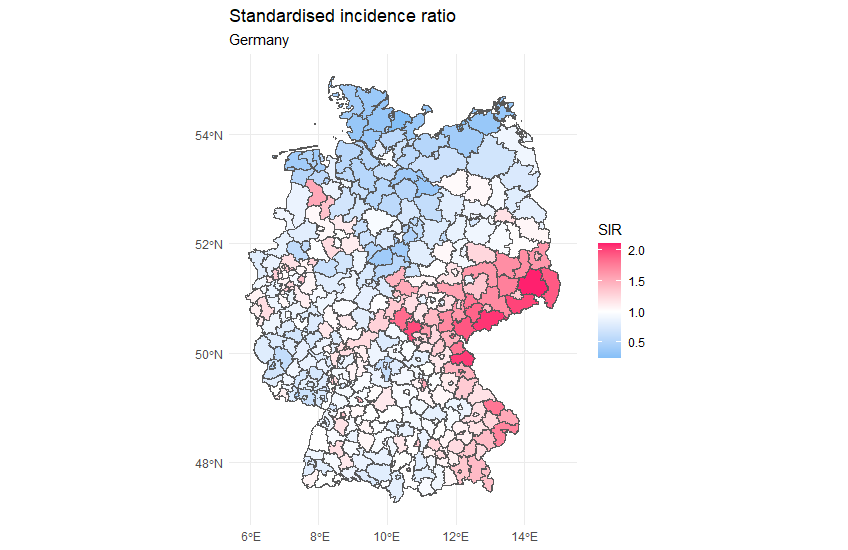
\includegraphics[width = 1.2\textwidth]{sir_germany.png}
  \caption{The standardised incidence ratio for Germany based on the data of the 24th of March 2021}
  \label{sirgermany}
\end{figure}
\subsection{Standardised Incidence Ratio for Norway}
Looking at the standardised incidence rate for Norway, a standardised incidence rate of less than 1 can be seen for most municipalities north of Trondheim. In the southern parts of Norway there are several municipalities with a rate above 1, for example the standardised incidence rate around the capital Oslo is around 2. However, the two small municipalities, Hyllestad and Ulvik, have the highest standardised incidence rate in Norway. In Hyllestad, 95 of 1328 people have been infected with Covid-19 so far, while in Ulvik, 134 of 1080 people have been infected so far. \\
The SIR in Hyllestad is around 4.5, following an outbreak in a shipyard in autumn 2020 \cite{newspaper1}, while Ulvik has a ratio of around 8, following an outbreak of the UK variant of Covid-19. According to the head of the municipality, Hans Petter Thorbjørnsen, the infections are thought to have spread through children \cite{newspaper2}. See Figure~\ref{sirnorway} for more information.
% \begin{figure}[H]
%   \centering
%   \includesvg[width = 1.2\textwidth]{sir_norway.svg}
%   \caption{The standardised incidence ratio for Norway based on the data of the 24th of March 2021}
%   \label{sirnorway}
% \end{figure}
\begin{figure}[H]
  \centering
  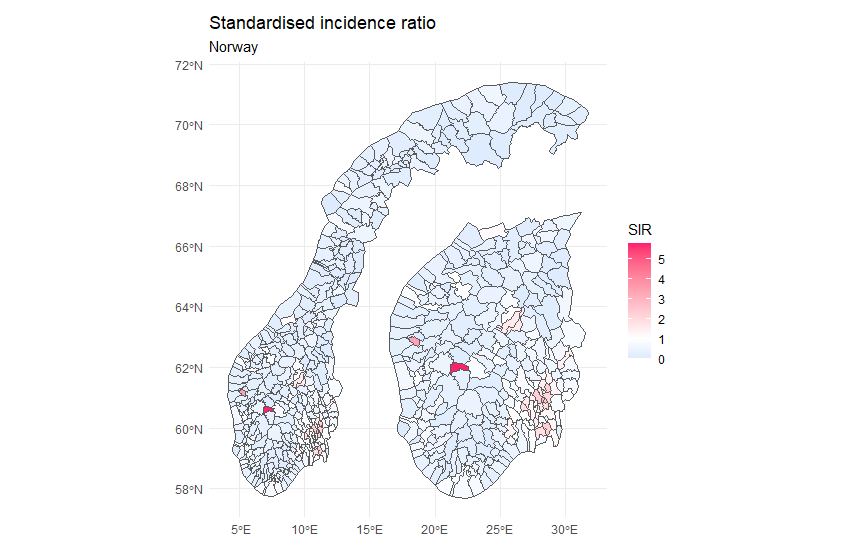
\includegraphics[width = 1.2\textwidth]{sir_norway.png}
  \caption{The standardised incidence ratio for Norway based on the data of the 24th of March 2021}
  \label{sirnorway}
\end{figure}
Because the high numbers from two small municipalities complicate the interpretation of Figure~\ref{sirnorway}, Figure~\ref{sirnorwaylog} shows the SIR on a log10 scale. It is now clearer that the standardized incidence ratio is below 1 in most parts of Norway, but that there is a higher risk in the region around Oslo.
% \begin{figure}[H]
%   \centering
%   \includesvg[width = 1.2\textwidth]{sir_norway_log.svg}
%   \caption{The log10 standardised incidence ratio for Norway based on the data of the 24th of March 2021}
%   \label{sirnorway}
% \end{figure}
\begin{figure}[H]
  \centering
  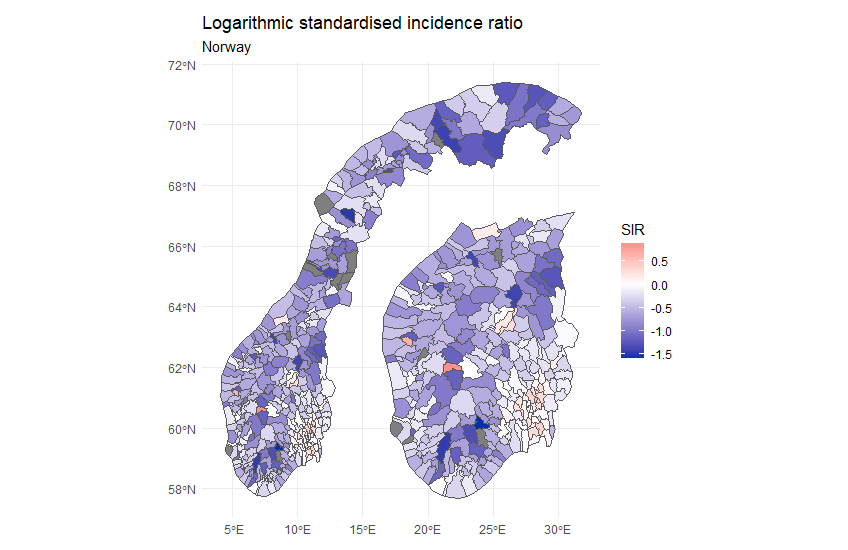
\includegraphics[width = 1.2\textwidth]{sir_norway_log.png}
  \caption{The log10 standardised incidence ratio for Norway based on the data of the 24th of March 2021}
  \label{sirnorwaylog}
\end{figure}
\clearpage
\section{Spatial Models}
After looking at the standardised incidence rates for the countries of interest, the next step is to take a closer look at the current figures for the respective countries. Spatial models are used to try to extract the factors that cause some populations to be at higher risk than other populations. Three different types of models are used for each country:
\begin{itemize}
    \item[1.] The Besarg-Yollie-Mollie Model
    \item[2.] Besags Proper Spatial Model
    \item[3.] The Leroux-Model
\end{itemize}
All of these models were computed using the INLA \cite{rinla} R package. \\
To specify each type of model, the code shown in Listing~\ref{codeModels} can be used. \\
Three measures are used to compare the models, the DIC, the WAIC and the CPO. \\
For all countries, the models were computed with
\begin{itemize}
    \item[1.] only the demographic variables as covariates
    \item[2.] only the infrastructural variables as covariates
    \item[3.] both, demographic and infrastructural variables, as covariates
    \begin{itemize}
        \item[3.1] Without variable selection
        \item[3.2] With variable selection
    \end{itemize}
\end{itemize}
For each model type, different values for the penalised prior were tried. As this resulted in a large number of models, only the model with the best performance for each model class is examined in more detail. \\
The models were compared using the mean absolute error. For this, 20\% of the observations were removed from the training and used for testing instead. The predicted number of infections for these municipalities was then compared to the actual numbers.
\\
Finally, due to the amount of covariates, forwards and backwards stepwise variable selection was performed with the intention of obtaining a model that fits the data well and at the same time is relatively easy to interpret. This can be done with the R package \texttt{INLAutils} \cite{inlautils}, as shown in Listing~\ref{codeSelection}. Backwards as well forwards variable selection was performed.\\
A list of all calculated models along with their performance measures is provided in the appendix.
\subsection{Model Selection}
Before the models are computed, however, the distribution that fits the number of cases must first be found. For this, the function \texttt{descdist()} from the \texttt{fitdistrplus} R package is used. The Cullen and Frey graph can be used to give an initial idea of which distributions fit the data, in this case the number of infections, reasonably well depending on the kurtosis and the square of the skewness. \\
The plots for Germany and Norway can be seen in Figure~\ref{cf_germany} and Figure~\ref{cf_norge}.
% \begin{figure}[H]
%     \centering
%     \includesvg[width = 0.8\textwidth]{cf_germany.svg}
%     \caption{The Cullen and Frey graph for Germany}
%     \label{cf_germany}
% \end{figure}
\begin{figure}[H]
    \centering
    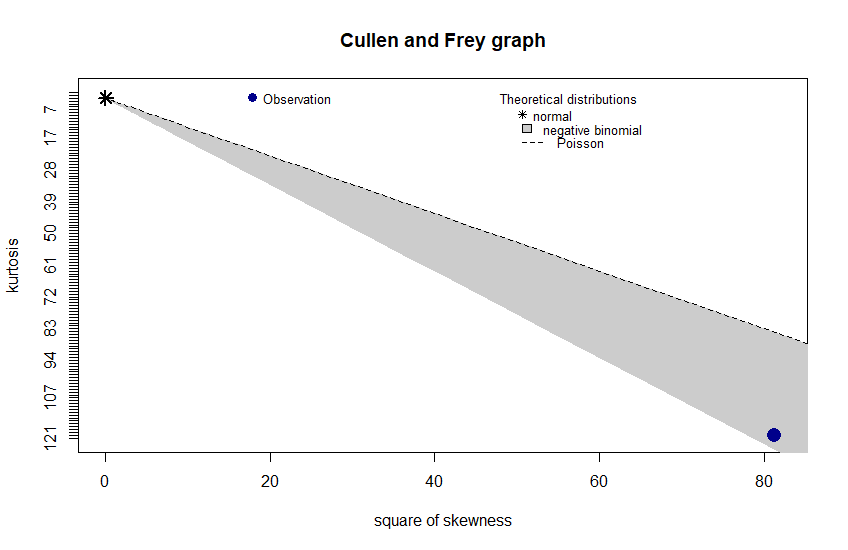
\includegraphics[width = 0.8\textwidth]{cf_germany.png}
    \caption{The Cullen and Frey graph for Germany}
    \label{cf_germany}
\end{figure}
% \begin{figure}[H]
%     \centering
%     \includesvg[width = 0.8\textwidth]{cf_norge.svg}
%     \caption{The Cullen and Frey graph for Norway}
%     \label{cf_norge}
% \end{figure}
\begin{figure}[H]
    \centering
    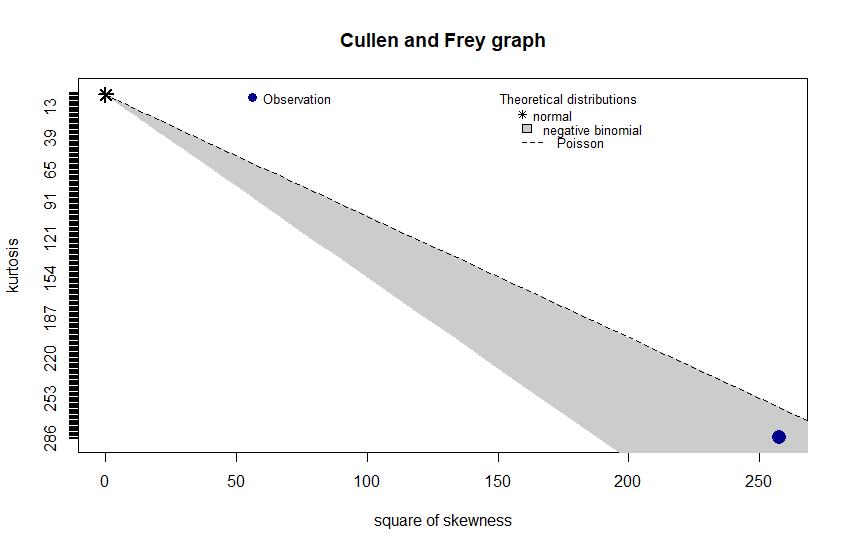
\includegraphics[width = 0.8\textwidth]{cf_norge.png}
    \caption{The Cullen and Frey graph for Norway}
    \label{cf_norge}
\end{figure}
Next, a negative binomial distribution, a normal distribution, and a Poisson distribution are fitted to the data using the maximum likelihood method. The negative binomial fits for both countries can be seen in Figure~\ref{fitNegbinomGermany} and Figure~\ref{fitNegbinomNorway}. The fits for the normal and Poisson distribution for both countries, are shown in the Appendix in Figure~\ref{fitNormalGermany}, Figure~\ref{fitPoissonGermany}, Figure~\ref{fitNormalNorway} and Figure~\ref{fitPoissonNorway}.
% \begin{figure}[H]
%     \centering
%     \includesvg[width = 0.8\textwidth]{fit_nbinom_germany.svg}
%     \caption{A negative binomial fit to the number of cases in German municipalities}
%     \label{fitNegbinomGermany}
% \end{figure}
\begin{figure}[H]
    \centering
    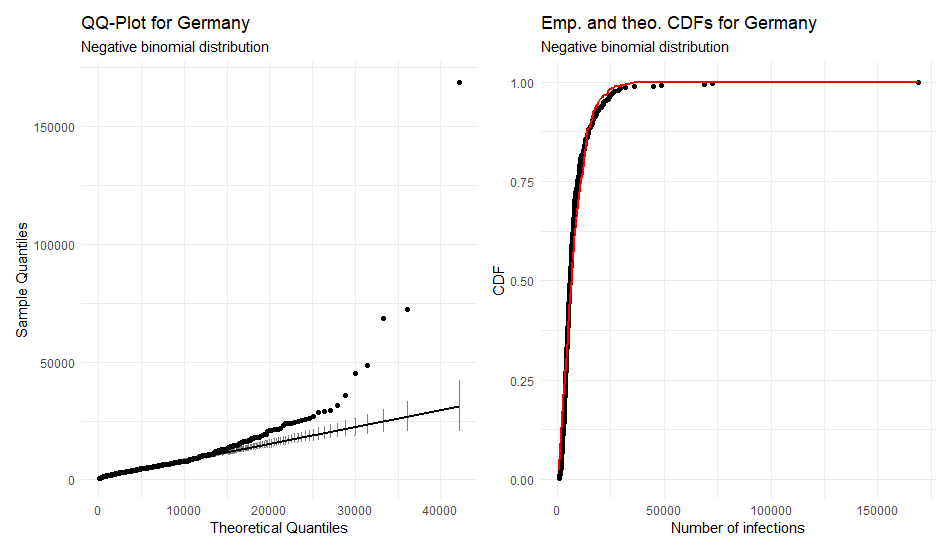
\includegraphics[width = 0.8\textwidth]{fit_nbinom_germany.png}
    \caption{A negative binomial fit to the number of cases in German municipalities}
    \label{fitNegbinomGermany}
\end{figure}
% \begin{figure}[H]
%     \centering
%     \includesvg[width = 0.8\textwidth]{fit_nbinom_norway.svg}
%     \caption{A negative binomial fit to the number of cases in Norwegian municipalities}
%     \label{fitNegbinomNorway}
% \end{figure}
\begin{figure}[H]
    \centering
    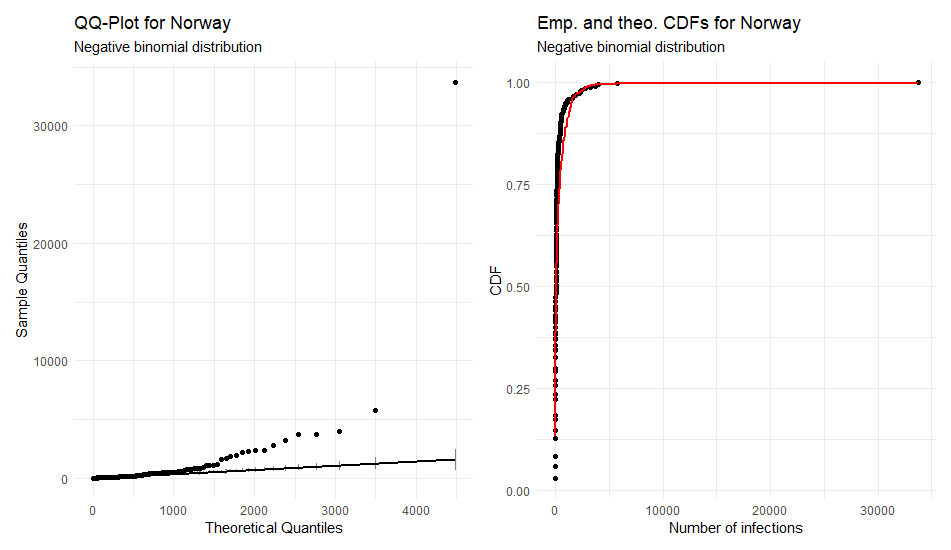
\includegraphics[width = 0.8\textwidth]{fit_nbinom_norway.png}
    \caption{A negative binomial fit to the number of cases in Norwegian municipalities}
    \label{fitNegbinomNorway}
\end{figure}
Lastly, the AIC was calculated for fitting a normal distribution to the data, a Poisson distribution to the data and a negative binomial distribution to the data. The values can be seen in Table~\ref{aic}. Afterwards, the negative binomial distribution was chosen as the distribution of the target variable in both cases. \\
\begin{table}[H] 
\caption{The AIC for different distributions for Germany and Norway \label{aic}}
\begin{tabular}{l l r}
\toprule
\textbf{Country}	& \textbf{Distribution}	& \textbf{AIC} \\
\midrule
Germany & Normal & 8360 \\
Germany & Poisson & 2148100 \\
Germany & Negative Binomial & 7731 \\
Norway & Normal & 6166 \\
Norway & Poisson & 366181 \\
Norway & Negative Binomial & 4086 \\
\bottomrule
\end{tabular}
\end{table} 
The poor fit for the Poisson distribution can be explained by looking at the range of the number of confirmed cases in a given municipality. For Germany, this number ranges from 508 to 137634 (as of March 18, 2021), while for Norway, the number ranges from 0 to 24905 (as of March 20, 2021). This results in a mean and standard deviation for Germany of 6617 and 9014, respectively. For Norway, the values for these metrics are 236 and 1389.
\subsection{Spatial Models for Germany}
First, a look is taken at the spatial models calculated for Germany. These models are based on data from 24 March 2021, when 2.695.037 people in Germany were confirmed infected with Covid-19. The five municipalities with the most infections are shown in Table~\ref{top5germany}.
\begin{table}[H] 
\caption{The municipalities with the most infections as of March 24th 2021. \label{top5germany}}
\begin{tabular}{l r r}
\toprule
\textbf{Municipality}	& \textbf{Population}	& \textbf{Number of infections} \\
\midrule
SK Berlin & 3644826 & 141639   \\     
SK Hamburg & 1841179 & 58661   \\
SK Munich & 1471508 & 57690   \\
SK Cologne & 1085664 & 37592   \\
Region Hannover & 1157624 & 36241   \\
\bottomrule
\end{tabular}
\end{table}
\subsubsection{Demographic Models}\label{sssec:demoGermany}
The model with the best performance based on the demographic variables was a Leroux model computed using the formula in Listing~\ref{codeDemoGermany}. The variables used for this model were the percentages of the vote for the six biggest German political parties. \\
The performance measures of this model and the best-performing BYM2 and Besag proper models are shown in Table~\ref{demoGermany}. 
\begin{table}[H] 
\caption{The performance measures for the best performing demographic model of each type. \label{demoGermany}}
\begin{tabular}{l r r r r}
\toprule
\textbf{Model}	& \textbf{DIC}	& \textbf{WAIC} & \textbf{CPO} & \textbf{MAE}\\
\midrule
Besag  & 4916 & 4919 & -2719 &  193968 \\
BYM2 & 4682 & 4670 & -2726 &  193922\\
Leroux & 4728  & 4753 & -3005 & 191965\\
\bottomrule
\end{tabular}
\end{table}
The summary of the fixed effects is shown in Table~\ref{fixedDemoGermany}. To compute the posterior mean of the coefficients, the code shown in Listing~\ref{codePosteriorMean} can be used. \\
To obtain a credibility interval of the fixed effects on the transformed scale, the code in Listing~\ref{codeCredibility} can be used. \\
\begin{table}[H] 
\caption{The fixed effects for the Leroux model. Values are rounded. A $^*$ denotes a significant effect.\label{fixedDemoGermany}}
\begin{tabular}{l r r r r c}
\toprule
\textbf{Variable}	& \textbf{Mean}	& \textbf{exp(mean$_{\hbox{p}}$)} & \textbf{exp(q0025$_{\hbox{p}}$)} & \textbf{exp(q0975$_{\hbox{p}}$)} & \textbf{sig.}\\
\midrule
(Intercept) & -0.07468 & 0.9282 & 0.8976 & 0.9594 &\\
afd & 0.1230 & 1.134& 0.9820 & 1.302 &$^*$\\
FDP & -0.01211 & 0.9881& 0.9515 & 1.026 &$^*$\\
Gruene & -0.1363 & 0.8750& 0.7555 & 1.008 6$^*$\\
SPD & -0.1702 & 0.8443 & 0.7749 & 0.9179 &\\
Union & -0.1714 & 0.8453& 0.7175 & 0.9889 &\\
die\_linke & -0.2159 & 0.8067 & 0.7353 & 0.8830 &\\
\bottomrule
\end{tabular}
\end{table}
The posterior mean of the exponentiated intercept implies a -7.2\% risk rate across Germany with a credibility interval ranging from -10.2\% to -4.1\%. However, this coefficient is not significant. \\
This summary shows that especially people who come from regions where the AfD gets a higher share of the vote have a higher risk of contracting Covid-19. In Figure~\ref{sirgermany}, regions in eastern Germany often had a higher SIR. These are also the regions where the AfD tends to perform better in elections. The connection between the two can be attributed to the fact that the AfD is a right-wing party that openly criticises the measures taken to prevent the spread of the coronavirus. As a result, a large proportion of people who vote for the AfD do not take the measures seriously either and refuse to keep a safe distance or wear a mask in public spaces. \\
A one standard deviation increase for the AfD leads to a risk increase of about 13.4\%. The only other party with a posterior mean close to 1 is the liberal FDP, which is known for its capitalist views. However, it is still below 1. An increase of 1 standard deviation leads to a risk reduction of 1.8\%. \\
As for the rest of the parties, they are either the leading party in Germany (Union) or left-wing oriented (SPD, the Greens and the Left). People who vote for left-wing parties may respect the Corona rules more and show more consideration for other people.
As this was the overall best-performing spatial model for Germany, a look is taken at the posterior means $\pmb{\zeta} = \exp{\left(\xi\right)}$ of the area-specific risks. Since the uncertainty associated with them can also be mapped, the posterior probability $\mathbb{P}\left(\zeta_i > 1|y\right)$ is visualised as well. In Figure~\ref{posteriorGermany}, it can be seen that the relative risk is above 1 for large parts of Germany, except for most of northern Germany and some parts in the south of the country. The posterior probability is highest for parts of North Rhine-Westphalia, home to Germany's most populous metropolitan area, the Ruhr area, and for Saxony and Thuringia, both political strongholds of the AfD. The higher numbers in Bavaria can be explained by the large common borders with Austria and the Czech Republic, two countries that were more affected by the pandemic. Many people cross these borders because of tourism and many guest workers come from the Czech Republic to work on agricultural land in Bavaria, which resulted in several Covid-19 outbreak events.
\begin{figure}[H]
    \centering
    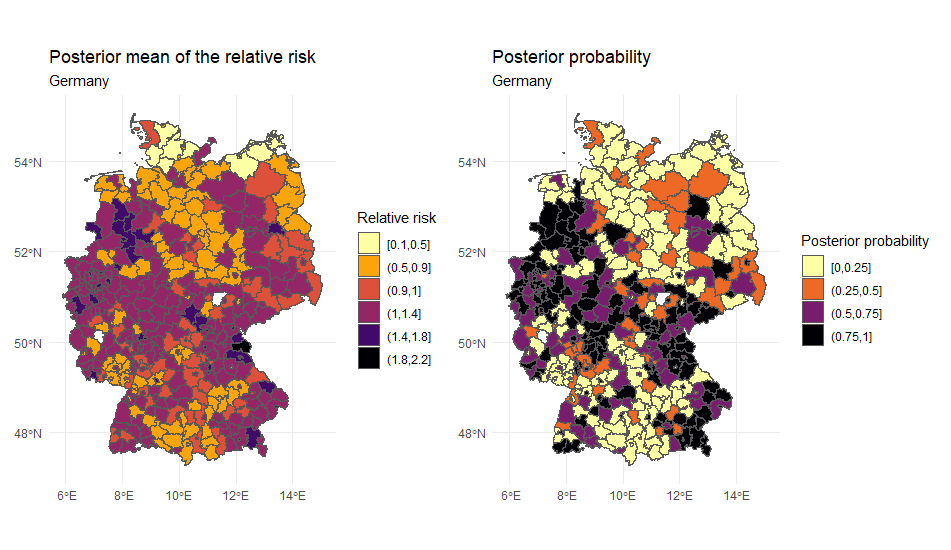
\includegraphics[width = \textwidth]{posterior_germany.png}
    \caption{Posterior mean of the area-specific risk and the posterior probability.}
    \label{posteriorGermany}
\end{figure}
% \begin{figure}[H]
%     \centering
%     \includesvg[width = textwidth]{posterior_germany.svg}
%     \caption{A negative binomial fit to the number of cases in Norwegian municipalities}
%     \label{nb_norge}
% \end{figure}
Compared to the standardised incidence rate in Germany, shown in Figure~\ref{sirgermany}, it can be seen that the parts of Germany with the lowest SIR, Northern Germany, are also the parts of Germany with the lowest relative risk. Saxony had the highest SIR and also has an increased relative risk. Most parts of Germany that had an SIR of around 1 have a relative risk between 1 and 1.4.
\subsubsection{Infrastructure Models}\label{sssec:infraGermany}
When it comes to the models based on the infrastructural variables, a BYM2 model performed the best. It was computed using formula in Listing~\ref{codeInfraGermany}. \\
The performance measures of this model and the best-performing Besag proper and Leroux model are shown in Table~\ref{infraGermany}
\begin{table}[H] 
\caption{The performance measures for the best performing infrastructure model of each type. \label{infraGermany}}
\begin{tabular}{l r r r r}
\toprule
\textbf{Model}	& \textbf{DIC}	& \textbf{WAIC} & \textbf{CPO} & \textbf{MAE}\\
\midrule
Besag & 4749 & 4745 & -2799 & 194009\\
BYM2 & 4635 & 4620 & -2758 & 193472\\
Leroux & 4785 & 4823 & -3444 & 1947560\\
\bottomrule
\end{tabular}
\end{table}
The values of the covariates are shown in Table~\ref{fixedInfraGermany}.
\begin{table}[H] 
\caption{The fixed effects for the BYM2 model. Values are rounded. A $^*$ denotes a significant effect.\label{fixedInfraGermany}}
\begin{tabular}{l r r r r c}
\toprule
\textbf{Variable}	& \textbf{Mean}	& \textbf{exp(mean$_{\hbox{p}}$)} & \textbf{exp(q0025$_{\hbox{p}}$)} & \textbf{exp(q0975$_{\hbox{p}}$)} & \textbf{sig.}\\
\midrule
(Intercept) & -0.07373 & 0.9289 & 0.9159 & 0.9421 &\\
shops & 0.3860 & 1.479 & 1.197 & 1.808 &$^*$\\
hairdresser & 0.1123 & 1.122 & 0.9655 & 1.296 &$^*$\\
marketplace & 0.04187 & 1.043 & 0.9846 & 1.104 &$^*$\\
schools & 0.02157 & 1.023 & 0.9199 & 1.135 &$^*$\\
nursing\_home & 0.01399 & 1.014 & 0.9879 & 1.042 &$^*$\\
aerodrome & 0.01273 & 1.013 & 0.9648 & 1.063 &$^*$\\
bakeries & 0.008426 & 1.011 & 0.8684 & 1.171 &$^*$\\
sport & 0.007894 & 1.009 & 0.9374 & 1.084& $^*$\\
office & 0.005687 & 1.006 & 0.9533 & 1.061 &$^*$\\
retail & -0.0028888 & 0.9977 & 0.9317 & 1.067 &$^*$\\
place\_of\_ & \multirow{2}{*}{-0.005710} & \multirow{2}{*}{0.9945} & \multirow{2}{*}{0.9562} & \multirow{2}{*}{1.034} &\multirow{2}{*}{$^*$}\\
worship &  \\
higher\_ & \multirow{2}{*}{-0.03179} & \multirow{2}{*}{0.9689} & \multirow{2}{*}{0.9324} & \multirow{2}{*}{1.006} &\multirow{2}{*}{$^*$}\\
education \\
clinic & -0.03258 & 0.9683 & 0.9154 & 1.023 &$^*$\\
entertainment & -0.03454 & 0.9676 & 0.8656 & 1.078 &$^*$\\
platform & -0.05867 & 0.9434 & 0.8913 & 0.9976 &\\
restaurant & -0.1990 & 0.8213 & 0.7206 & 0.9316 &\\
kindergarten & -0.2268 & 0.7993 & 0.6871 & 0.9243 &\\
\bottomrule
\end{tabular}
\end{table}
Some findings from these results are that shops, defined as supermarkets, convenience stores and drugstores, hairdressers, marketplaces, schools, nursing homes and bakeries, among others, increase the risk of infection. The two highest are shops and hairdressers, where a 1 standard deviation increase leads to a 47.9\% increase in risk in the case of shops and a 12.2\% increase in risk for hairdressers. It should not be surprising that shops in particular increase the risk of infection, as people tend to congregate there and people living in areas where a supermarket is nearby may prefer to go shopping more often to buy fresh produce rather than just once a week when a supermarket is further away. \\
In Germany, there was a big discussion about whether hairdressers should be allowed to stay open during lockdowns, as they were forced to close and could only work when there was no lockdown. Seeing how much hairdressers increase the risk of infection, it might have been a wise decision not to allow them to continue working during a closure. \\
Finally, the number of schools in a given community also increases the risk of infection. An increase of 1 standard deviation increases the risk by about 2.3\%.
\\
There are also effects that have a posterior mean of less than 1, suggesting that they reduce the risk of infection. However, this is not necessarily the case, as it is probably safer for a person to stay at home than to go to a restaurant, for example. It is interesting to note, however, that the two lowest posterior means were observed for restaurants and kindergartens. In the case of restaurants, this could be due to the fact that during most of the period restaurants were either only allowed to serve take-away food or had very strict hygiene rules. The low value could indicate that these measures worked as intended. \\
For the kindergartens, the reason could be that they were also closed most of the time and the children therefore stayed at home with their families and did not interact with other children.
\subsubsection{Combined Models}
Finally, models are considered that include both the infrastructural and demographic covariates. Due to the amount of variables, all models run are based on variable selection. \\
The best performing model was again a BYM2 model, run with the formula shown in Listing~\ref{codeBothGermany}. \\
The performance measures of the computed models are shown in Table~\ref{allGermany}.
\begin{table}[H] 
\caption{The performance measures for the best performing demographic + infrastructure model of each type. \label{allGermany}}
\begin{tabular}{l r r r r}
\toprule
\textbf{Model}	& \textbf{DIC}	& \textbf{WAIC} & \textbf{CPO} & \textbf{MAE}\\
\midrule
Besag&  4755 & 4721 & -2756 & 198553\\
BYM2 & 4753 & 4774 & -2776 & 198461\\
Leroux & 4847 & 4818 & -2684 & 204102 \\
\bottomrule
\end{tabular}
\end{table}
The fixed effects are shown in Table~\ref{fixedAllGermany}.

\begin{table}[H] 
\caption{The fixed effects for the BYM2 model. Values are rounded. A $^*$ denotes a significant effect.\label{fixedAllGermany}}
\begin{tabular}{l r r r r c}
\toprule
\textbf{Variable}	& \textbf{Mean}	& \textbf{exp(mean$_{\hbox{p}}$)} & \textbf{exp(q0025$_{\hbox{p}}$)} & \textbf{exp(q0975$_{\hbox{p}}$)} & \textbf{sig.}\\
\midrule
(Intercept) & -0.0716 & 0.9309 & 0.9168 & 0.9450 &\\
afd & 0.2528 & 1.288 & 1.222 & 1.357 &$^*$\\
pop\_dens & 0.09614 & 1.101 & 1.055 & 1.148 &$^*$\\
welfare\_ & \multirow{2}{*}{0.07515} & \multirow{2}{*}{1.079} & \multirow{2}{*}{1.004} & \multirow{2}{*}{1.157}&\multirow{2}{*}{$^*$} \\
recipients\\
sport & 0.05575 & 1.058 & 0.9945 & 1.124 &$^*$\\
schools & 0.03926 & 1.041 & 0.9485 & 1.140 &$^*$\\
nursing\_home & 0.008492 & 1.009 & 0.9856 & 1.032&$^*$ \\
office & -0.007482 & 0.9928 & 0.9510 & 1.036 &$^*$\\
log(trade\_tax) & -0.007660 & 0.9924 & 0.9695 & 1.016&$^*$ \\
place\_of\_ & \multirow{2}{*}{-0.01141} & \multirow{2}{*}{0.9888} & \multirow{2}{*}{0.9557} & \multirow{2}{*}{1.023} &\multirow{2}{*}{$^*$}\\
worship\\
platform & -0.02052 & 0.9800 & 0.9322 & 1.029 &$^*$\\
kindergarten & -0.02174 &  0.9799 & 0.8812 & 1.087 &$^*$\\
FDP & -0.03154 & 0.9691 & 0.9340 & 1.005 &$^*$\\
SPD & -0.03197 & 0.9688 & 0.9288 & 1.010 &$^*$\\
entertainment & -0.03963 & 0.9619 & 0.8891 & 1.039 &$^*$\\
bakeries & -0.06149 & 0.9419 & 0.8412 & 1.051 &$^*$\\
die\_linke & -0.08336 &  0.9204 & 0.8697 & 0.9734\\
\bottomrule
\end{tabular}
\end{table}
According to this model, the three biggest driving factors are the percentage of votes the AfD receives, the population density and the number of welfare recipients in a municipality. The influence of the AfD has already been discussed in section~\ref{sssec:demoGermany}, only in this case a 1 standard deviation increase leads to a risk increase of 28.8\%. Regarding population density, it can be said that if it increases by 1 standard deviation, the risk of infection increases by 10.1\%. The more people are concentrated per square kilometre, the easier it is for a virus to spread because the distances between people become smaller. Other factors that positively influence the risk of infection are the number of sports facilities, the number of schools and the number of nursing homes, although the risk increase for the latter is only just above 0. Sports facilities are again a place where many people come together, and here, depending on the type of sport, there can also be more contact, which in turn favours the spread of a virus. The last effect worth mentioning is the logarithmic trade tax. If a region receives more revenue through trade tax, the risk of infection in that region decreases. Therefore, people in communities where there is less money are at higher risk. 
\subsection{Spatial Models for Norway}
Next, the same types of models are evaluated for Norway. These models are based on data from 24 March 2021, when 87537 people in Norway were confirmed infected with Covid-19. The five municipalities with the most infections are shown in Table~\ref{top5norway}.
\begin{table}[H] 
\caption{The municipalities with the most infections as of March 24th 2021. \label{top5norway}}
\begin{tabular}{l r r}
\toprule
\textbf{Municipality}	& \textbf{Population}	& \textbf{Number of infections} \\
\midrule
Oslo & 693494 & 26151 \\
Bergen & 283929 & 4738 \\
Drammen & 101386 & 3149 \\
Bærum & 127731 & 2834 \\
Lillestrøm & 85983 & 2779 \\
\bottomrule
\end{tabular}
\end{table}
\subsubsection{Demographic Models}
As with Germany, the best demographic model was again a Leroux model calculated using the formula shown in Listing~\ref{codeDemoNorway}. \\
The performance measures for all three models are shown in Table~\ref{demoNorway}. It is noticeable that the mean error in Norway is significantly smaller, suggesting that the models for Germany have greatly overestimated or underestimated the number of infections.
\begin{table}[H] 
\caption{The performance measures for the best performing demographic model of each type. \label{demoNorway}}
\begin{tabular}{l r r r r}
\toprule
\textbf{Model}	& \textbf{DIC}	& \textbf{WAIC} & \textbf{CPO} & \textbf{MAE}\\
\midrule
Besag  & 2396 & 2403 & -4369 & 10149 \\
BYM2 & 2224 & 2202 & -6793 & 10002\\
Leroux & 2225  & 2192 & -6810 & 8460\\
\bottomrule
\end{tabular}
\end{table}
All other performance measures for these models are also lower than for the models computed for Germany. \\
The effects of the covariates are shown in Table~\ref{fixedDemoNorway}.
\begin{table}[H] 
\caption{The fixed effects for the Leroux model. Values are rounded. A $^*$ denotes a significant effect.\label{fixedDemoNorway}}
\begin{tabular}{l r r r r c}
\toprule
\textbf{Variable}	& \textbf{Mean}	& \textbf{exp(mean$_{\hbox{p}}$)} & \textbf{exp(q0025$_{\hbox{p}}$)} & \textbf{exp(q0975$_{\hbox{p}}$)} & \textbf{sig.}\\
\midrule
(Intercept) & -1.040 & 0.3540 & 0.3173 & 0.3929 & \\
unemp\_total & 0.3371 & 1.406 & 1.192 & 1.645 & $^*$\\
unemp\_immg & 0.03737 & 1.042 & 0.8788 & 1.226 & $^*$\\
\bottomrule
\end{tabular}
\end{table}
The posterior mean of the section implies a risk rate of -64.6\%, however this effect is not significant. According to this model, the risk depends on only two factors, namely total unemployment and immigrant unemployment. A 1 standard deviation increase in total unemployment leads to a 40.6\% increase in risk and a 1 standard deviation increase in immigrant unemployment leads to a 4.2\% increase in risk. A possible explanation for this could be that the unemployed spend less time at home and instead move around more and thus have more contact with people, but this should be taken with a grain of salt.
\subsubsection{Infrastructure Models}
For the models based on the infrastructural variables, the best predictive performance was observed for a Besag model. The formula is shown in Listing~\ref{codeInfraNorway}. \\
The performance measure for the models are shown in Table~\ref{infraNorway}.
\begin{table}[H] 
\caption{The performance measures for the best performing infrastructure model of each type. \label{infraNorway}}
\begin{tabular}{l r r r r}
\toprule
\textbf{Model}	& \textbf{DIC}	& \textbf{WAIC} & \textbf{CPO} & \textbf{MAE} \\
\midrule
Besag  & 2326 & 2335 & -8405 & 11694 \\
BYM2 & 2218 & 2187 & -6532 & 11866\\
Leroux &  2230 & 2167 & -7128 & 12943\\
\bottomrule
\end{tabular}
\end{table}
The effect of the covariates are shown in Table~\ref{fixedInfraNorway}.
\begin{table}[H] 
\caption{The fixed effects for the Besag model. Values are rounded. A $^*$ denotes a significant effect.\label{fixedInfraNorway}}
\begin{tabular}{l r r r r c}
\toprule
\textbf{Variable}	& \textbf{Mean}	& \textbf{exp(mean$_{\hbox{p}}$)} & \textbf{exp(q0025$_{\hbox{p}}$)} & \textbf{exp(q0975$_{\hbox{p}}$)} & \textbf{sig.}\\
\midrule
(Intercept) & -1.061 & 0.3518 & 0.2437 & 0.4965 &\\
schools & 0.3253 & 1.407 & 0.9864 & 1.966 & $^*$\\
kindergarten & 0.2418 & 1.285 & 0.9825 & 1.663 & $^*$\\
pop\_dens & 0.1531 & 1.171 &  0.9733  & 1.406& $^*$\\
place\_of\_ & \multirow{2}{*}{0.03138} & \multirow{2}{*}{1.041} & \multirow{2}{*}{0.8053} & \multirow{2}{*}{1.335} & \multirow{2}{*}{$^*$}\\
worship\\
restaurant & 0.01374 & 1.044 & 0.6384 & 1.626 & $^*$\\
nursing\_home & 0.001030 & 1.002 & 0.9258 & 1.085& $^*$\\
office & -0.07424 & 0.9263 &  0.7991 & 1.084 & $^*$\\
shops & -0.5186 &0.6451 & 0.2793 & 1.303 & $^*$\\
\bottomrule
\end{tabular}
\end{table}
According to this model, schools, kindergartens, places of worship and nursing homes are infrastructural features that increase the risk of infection. In addition, higher population density also increases the risk of infection. Schools and kindergartens are the two biggest driving factors, as a 1 standard deviation increase in schools leads to a 40.7\% increase in risk and a 1 standard deviation increase in kindergartens leads to a 28.5\% increase in risk. The risk of schools and kindergartens is reflected in the Corona outbreak that occurred in Tromsø in early March 2021, where several infections have been linked to school classes and kindergartens \cite{tromsokorona}. A 1 standard deviation increase in population density leads to a 17.1\% increase in risk, and for places of worship and nursing homes, a 1 standard deviation increase leads to a 4.1\% and 0.2\% increase in risk, respectively. Finally, for restaurants, a 1 standard deviation increase leads to a 4.4\% increase in risk. Why restaurants do not have a large impact on the risk of infection has already been discussed in Section~\ref{sssec:infraGermany}
\\
For offices and shops, on the other hand, there is no increased risk of infection. For offices, one reason why they do not increase the risk could be that more and more people work from home and therefore there is less contact between people at office locations and thus no increased risk of infection. Finally, shops do not increase the risk of infection here, whereas in Germany they were one of the driving factors, as can be seen in Table~\ref{fixedInfraGermany}. Why this is so is difficult to say. Because of the lower infection numbers, there is of course less risk when people congregate in supermarkets, which may be an explanation, even if these are not driving factors of the pandemic in Norway. It could also mean that Norwegians are more likely to be careful to keep enough distance from each other. \\
Looking at the posterior mean relative risk, it can be seen that the region in and around the capital Oslo is most at risk, as the posterior mean of the relative risk can be as high as 6, with a posterior probability between 0.75 and 1. In addition, some municipalities around Bergen and Ulvik are also more at risk, with a relative risk of up to 3.4 and a posterior probability between 0.75 and 1. \\
The risk seems to be lowest in the parts north of Trondheim and south of Bodø, where the relative risk is mostly below 1. For many municipalities in Troms og Finnmark, the northernmost part of Norway, the posterior mean is also below 1, but for a few regions it is above 1 with posterior probabilities between 0.5 and 0.75 and 0.75-1.
\begin{figure}[H]
    \centering
    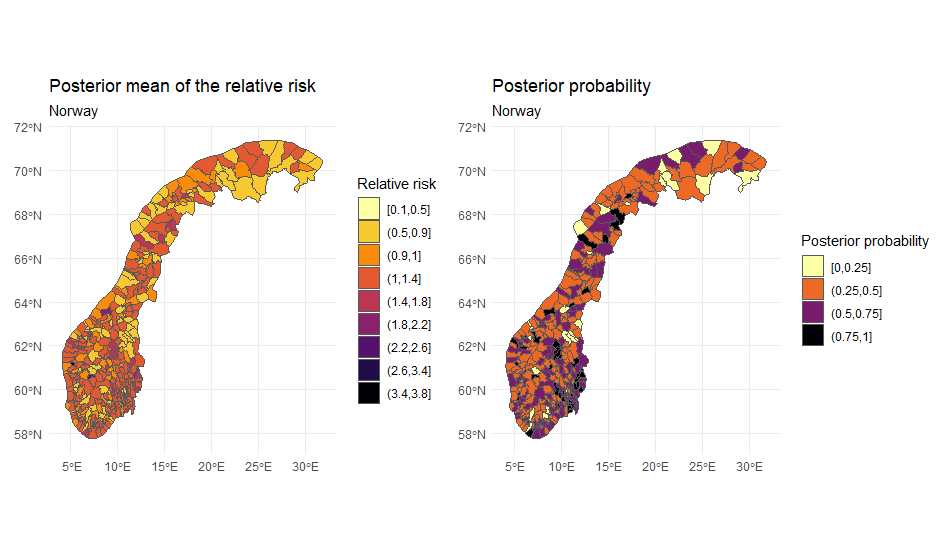
\includegraphics[width = \textwidth]{posterior_norway.png}
    \caption{Posterior mean of the area-specific risk and the posterior probability.}
    \label{posteriorNorway}
\end{figure}
% \begin{figure}[H]
%     \centering
%     \includesvg[width = textwidth]{posterior_norway.svg}
%     \caption{Posterior mean of the area-specific risk and the posterior probability.}
%     \label{posteriorNorway}
% \end{figure}
For better interpretability, the logarithmic posterior mean is shown in Figure~\ref{posteriorNorwayLog}.
\begin{figure}[H]
    \centering
    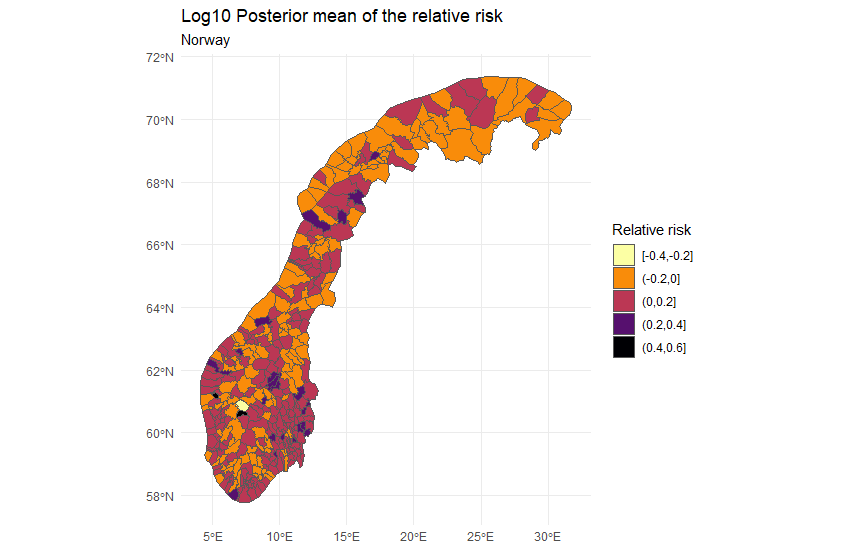
\includegraphics[width = \textwidth]{posterior_norway_log.png}
    \caption{Logarithmic posterior mean of the area-specific risk.}
    \label{posteriorNorwayLog}
\end{figure}
% \begin{figure}[H]
%     \centering
%     \includesvg[width = textwidth]{posterior_norway_log.svg}
%    \caption{Logarithmic posterior mean of the area-specific risk.}
%     \label{posteriorNorwayLog}
% \end{figure}
Comparing the log relative risk with the log standardised incidence ratio in Figure~\ref{sirnorwaylog}, these two are quite similar. For most parts of Norway, the risk is at or below 0, while there is an increased risk in the Oslo region. However, there are a few municipalities that have a log-standardised incidence ratio of about 0, but a higher log-relative risk than this. Most of these are located in southern Norway, but a few are scattered throughout the rest of the country.
\subsubsection{Combined Models}
For the models containing variables related to the demographic of Norway and the infrastructure, again a Besag model performed the best. Its formula can be seen in Listing~\ref{codeBothNorway}. \\
The performance measures for the models are shown in Table~\ref{bothNorway}
\begin{table}[H] 
\caption{The performance measures for the best performing demographic + infrastructure model of each type. \label{bothNorway}}
\begin{tabular}{l r r r r}
\toprule
\textbf{Model}	& \textbf{DIC}	& \textbf{WAIC} & \textbf{CPO} & \textbf{MAE} \\
\midrule
Besag  & 2352 & 2355 & -6939 & 13036 \\
BYM2 & 2215 & 2184 & -6406 & 13932\\
Leroux &  2229 & 2193 & -7677 & 14841\\
\bottomrule
\end{tabular}
\end{table}
The fixed effects are shown in Table~\ref{fixedAllNorway}.
\begin{table}[H] 
\caption{The fixed effects for the Besag model. Values are rounded. A $^*$ denotes a significant effect.\label{fixedAllNorway}}
\begin{tabular}{l r r r r c}
\toprule
\textbf{Variable}	& \textbf{Mean}	& \textbf{exp(mean$_{\hbox{p}}$)} & \textbf{exp(q0025$_{\hbox{p}}$)} & \textbf{exp(q0975$_{\hbox{p}}$)} & \textbf{sig.}\\
\midrule
(Intercept) & -1.068 & 0.3484 & 0.2478 & 0.4736 &\\
construction\_ & \multirow{2}{*}{0.1873} & \multirow{2}{*}{1.234} & \multirow{2}{*}{0.7946} & \multirow{2}{*}{1.834} & \multirow{2}{*}{$^*$} \\
pt\_work \\
clinic & 0.1855 & 1.266 & 0.6488 & 2.241 & $^*$\\
pop\_dens & 0.1717 & 1.194 & 0.9703 & 1.455 & $^*$\\
unemp\_tot & 0.1559 & 1.170 & 1.057 & 1.292 & $^*$\\
schools & 0.0978 & 1.117 & 0.8074 & 1.507 & $^*$\\
sex & 0.04402 & 1.046 & 0.9426 & 1.158 & $^*$\\
restaurant & 0.03072 & 1.079 & 0.5717 & 1.855 & $^*$\\
higher\_& \multirow{2}{*}{-0.05942} & \multirow{2}{*}{0.9443} & \multirow{2}{*}{0.8295} & \multirow{2}{*}{1.069} & \multirow{2}{*}{$^*$}\\
education\\
median\_age & -0.1147 & 0.8929 & 0.8015 & 0.9910 & \\
workers\_ft\_ & \multirow{2}{*}{-0.5200} & \multirow{2}{*}{0.6403} & \multirow{2}{*}{0.2784} & \multirow{2}{*}{1.259} & \multirow{2}{*}{$^*$}\\
work\\
\bottomrule
\end{tabular}
\end{table}
Some of these factors have already been discussed in the previous sections, so they will not be discussed in detail again. \\
The number of clinics, the number of part-time construction workers, the population density, total unemployment and the number of schools are the five biggest drivers of relative risk, as a 1 standard deviation increase in any of these factors leads to an increase in relative risk of 26.6\%, 23.4\%, 19.4\%, 17.0\% and 11.7\% respectively. That clinics increase the relative risk could be due to the fact that when there are more clinics in a community, more people who have symptoms go to a clinic and get tested, which naturally leads to more detected cases. In Norway, there has been some discussion about whether the number of foreign construction workers coming from countries with higher infection rates, such as Poland, could contribute to the spread of Covid-19. Since most of these are classified as part-time workers, this model suggests that this may be the case. \\
The other two factors that increase the risk are the proportion of women in a community and the number of restaurants. For the proportion of women, a 1 standard deviation increase leads to a 4.6\% increase in risk and for restaurants, a 1 standard deviation increase leads to a 0.8\% increase in risk. \\
The median age lowers the risk of infection, as an increase of 1 standard deviation lowers the relative risk by 9.8\%. This in turn means that people living in communities with a lower median age have a higher risk than people living in "older" communities. This could be due to the fact that younger people tend to be more mobile and have more contact with other people as a result of this increased movement, which in turn helps the virus spread.
\clearpage
\section{Spatio-Temporal Models}
\subsection{Spatio-Temporal Models for Germany}
\subsection{Spatio-Temporal Models for Norway}
\section{Predictive Models}
\subsection{Predictive Models for Germany}
\subsection{Predictive Models for Norway}